\section{Métodos elementales de conteo}\label{metodos-elementales-de-conteo}

A lo largo de este tema vamos a ver cómo computar las diferentes formas en las que se puede dispone de varios elementos concretos y abstractos.
Antes de nada, vamos a redefinir las operaciones suma y producto para trabajar de forma más eficiente con ellas.

\subsection{Principio de la suma}\label{principio-de-la-suma}

\[A \cap B = \emptyset \Rightarrow |A \cup B| = |A| + |B|\]

Dados dos conjuntos $A$ y $B$ disjuntos, es decir, que $a \neq b, \forall a \in A, b \in B$, podemos contar los elementos de ambos conjuntos empezando a contar todos los de $A$ y seguir con los de $B$ hasta llegar al total.
Sin embargo, si conocemos la cardinalidad de los conjuntos, podemos tomar el atajo de simplemente sumarlas.
Vamos a aplicar este princpio a la combinatoria para encontrar el número de formas de las que se pueden realizar varias tareas siempre que dichas tareas sean incompatibles.
Por ejemplo, podemos usar este principio para contar las diferentes formas de elegir manzanas de dos cestos, ya que no podemos coger manzanas de dos cestos a la vez con una mano.
De esta forma, si en el cesto $A$ tenemos 4 manzanas y en el $B$, 3, podemos coger las manzanas de 7 formas diferentes.

\subsection{Principio de inclusión-exclusión}\label{principio-de-inclusion-exclusion}

Si los conjuntos sobre cuyas cardinalidades estamos aplicando el principio de la suma no son incompatibles, debemos usar la forma general del princpio de inclusión-exclusión para calcular la suma de las mismas:

\[|A \cup B| = |A| + |B| - |A \cap B|\]

\begin{figure}[h!]
\begin{center}
\begin{tikzpicture}
	\begin{scope}
		\clip             (180:1cm) circle (2cm);
		\fill[light-gray] (0:1cm)   circle (2cm);
	\end{scope}

	\draw (180:1cm) circle (2cm) node [text=black, label={[label distance=0.5cm]180:$A$}] {};
	\draw (0:1cm)   circle (2cm) node [text=black, label={[label distance=0.5cm]000:$B$}] {};
	\draw                        node [text=black]                                        {$A \cap B$};
\end{tikzpicture}
\ \ \ \ \ \ \ \ \ \ %
\begin{tikzpicture}
	\begin{scope}
		\clip             (90:1.5cm)  circle (2cm);
		\fill[light-gray] (180:1cm)   circle (2cm);
	\end{scope}
	\begin{scope}
		\clip             (180:1cm) circle (2cm);
		\fill[light-gray] (0:1cm)   circle (2cm);
	\end{scope}
	\begin{scope}
		\clip             (0:1cm)    circle (2cm);
		\fill[light-gray] (90:1.5cm) circle (2cm);
	\end{scope}
	\begin{scope}
		\clip             (90:1.5cm) circle (2cm);
		\clip             (180:1cm)  circle (2cm);
		\fill[white]      (0:1cm)    circle (2cm);
	\end{scope}

	\draw (90:1.5cm) circle (2cm) node [text=black, label={[label distance=0.75cm]090:$A$}]               {};
	\draw (180:1cm)  circle (2cm) node [text=black, label={[label distance=0.75cm]210:$B$}]               {};
	\draw (0:1cm)    circle (2cm) node [text=black, label={[label distance=0.75cm]330:$C$}]               {};
	\draw                         node [text=black, label={[label distance=1.10cm]060:$A \cap C$}]        {};
	\draw                         node [text=black, label={[label distance=1.10cm]120:$A \cap B$}]        {};
	\draw                         node [text=black, label={[label distance=0.55cm]270:$B \cap C$}]        {};
	\draw                         node [text=black, label={[label distance=0.20cm]090:$A \cap B \cap C$}] {};
\end{tikzpicture}
\end{center}
\caption{Suma de dos y tres conjuntos. Los sectores blancos se suman y los grises se restan.}
\end{figure}

Por ejemplo, seguimos este principio para calcular el número de animales que o bien viven en la sabana ($A$) o son herbívoros ($B$) pero no ambos ($A \cap B$).
Este princpio es escalable a más conjuntos.
En el caso de tres, por ejemplo, tenemos la siguiente expresión:

\[|A \cup B \cup C| = |A| + |B| + |C| - |A \cap B| - |A \cap C| - |B \cap C| + |A \cap B \cap C|\]

Vemos que tenemos que sumar las uniones de números impares de conjuntos y restar las pares, por lo que podemos dar una forma general para este principio:

\[|A_1 \cup A_2 \cup \cdots \cup A_n| = \sum_{k=1}^{n} {(-1)}^{k+1} \cdot \sum_{1 \leq i_1 < \cdots < i_k \leq n} |A_{i_1} \cap A_{i_2} \cap \cdots \cap A_{i_n}|\]

\subsection{Principio del producto}\label{principio-del-producto}

\[A_1 \times A_2 \times \cdots \times A_3| = |A_1| \cdot |A_2| \cdots |A_n|\]

Además de dar una forma clara de calcular la cardinalidad del producto vectorial de varios conjuntos, este principio nos sirve para resolver problemas dividiendo la tarea en tareas consecutivas más sencillas.
Si cada tarea $A$ se puede de $i$ formas, cada tarea $A_i$ y su siguiente tarea $A_{i+1}$ se pueden resolver de $|A_i| \cdot |A_{i+1}|$ formas.
Este principio es escalable a cualquier número de conjuntos o tareas que queramos calcular.

\begin{figure}[h!]
\begin{center}
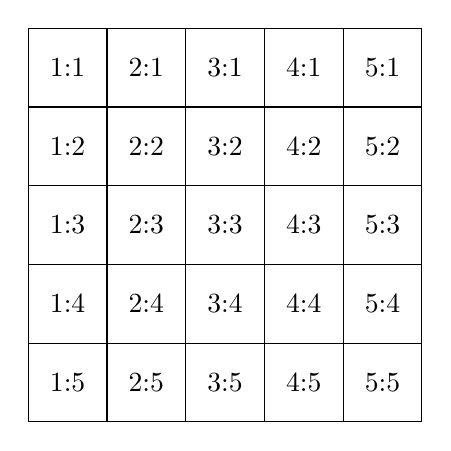
\begin{tikzpicture}
	\draw[thin, black] (0,0) grid (5,5);
	\foreach \x in {1,2,3,4,5}
		\foreach \y in {1,2,3,4,5}
			\pgfmathsetmacro\ycalc{int(6-\y)}
			\node at (\x-0.5,\y-0.5) {\x:\ycalc};
\end{tikzpicture}
\end{center}
\caption{Este tablero de 5 filas y 5 columnas tiene 25 casillas.}
\end{figure}

\subsection{Principio del palomar}\label{principio-del-palomar}

Supongamos que queremos repartir $p$ palomas en un palomar con $n$ huecos.
Lo lógico es asignar una paloma a cada uno de los huecos.
Sin embargo, si tenemos más palomas que huecos ($p >n$), necesariamente tendremos que asignar más de una paloma a alguno de los huecos.
Este principio puede servirnos para resolver problemas en los que queramos dividir $p$ elementos en $n$ partes si $p > n$.

\subsubsection{Principio del palomar generalizado}

Dado un palomar con $n$ huecos en el que queremos repartir $p$ palomas, cada hueco deberá contener necesariamente al menos $\frac{p}{n}$ palomas.
Lógicamente, tomaremos el número entero inmediatamente superior a $\frac{p}{n}$.
